
\documentclass[10pt,openany,a4paper]{article}
\usepackage{tikz, pgfplots, tkz-euclide,calc}
\usetikzlibrary{patterns,shapes.arrows,calc}
\usepackage{fancyhdr}
\usepackage{enumerate,enumitem}
\usepackage{cancel}
\usepackage{varwidth}

% TAMBAHKAN PACKAGE SENDIRI KALAU KURANG

\usepackage{geometry}
\geometry{
	left = 22mm,
	right = 22mm,
	top = 25mm,
	bottom = 25mm,
}
\usepackage{graphicx}
\usepackage{subcaption}
\usepackage{soul}
\usepackage{hyperref}
\usepackage{float}
\usepackage{setspace}
\usepackage{afterpage}
\usepackage{xcolor}
\usepackage[nosectionbib]{apacite}
\usepackage{lmodern}
\usepackage{mathtools}
\usepackage{upgreek}
\usepackage{siunitx}
% \usepackage{fontawesome5}
\usepackage{fontawesome6}
\usepackage{physics}
\usepackage{pdfpages}
\usepackage{hyperref}
\renewcommand{\baselinestretch}{1.3}
\usepackage{multicol}
\usepackage{hyperref,ragged2e,amsmath,multicol,gensymb,setspace,
fancyhdr,amsfonts,tikz,pgfplots,nccmath,enumerate,verbatim,amsthm,physics}
\usepgfplotslibrary{polar,fillbetween}
% Disable tikz externalization to avoid requiring -shell-escape
\usepgfplotslibrary{external}
\tikzexternalize[prefix=tikz/]
\tikzset{reuse path/.code={\pgfsyssoftpath@setcurrentpath{#1}}}
\usetikzlibrary{shapes.geometric,arrows}
\newcommand\mylog[1]{\mathop{{}^{#1}\mathrm{log}}}
\pgfplotsset{compat=1.15}
\pgfplotsset{my style/.append style={axis x line=middle, axis y line=
middle, xlabel={$x$}, ylabel={$y$}, axis equal }}
\usepackage{etoolbox}
% remove stray \makeatother
\newtheorem{defn}{Definisi}[section]
\newtheorem{teo}[defn]{Teorema}
\newtheorem{thm}{Teorema}[section]
\newtheorem{lemma}{Lemma}
\newtheorem{lemmas}[defn]{Lemma}
\newtheorem{cor}[defn]{Akibat}
\newtheorem{asumsi}[defn]{Asumsi}
\theoremstyle{definition}
\newtheorem{con}{Contoh}[section]
\theoremstyle{definition}
\theoremstyle{plain}
\newtheorem{prop}{Proposisi}[section]
\renewcommand{\proofname}{Bukti}
\renewcommand{\thethm}{\arabic{chapter}.\arabic{thm}}

\newcommand{\normlp}[1]{\left\|#1\right\|_{L^p_{\lambda}(0,T;H)}}% Fungsi norm (||x||)
\newcommand{\R}{\mathbb{R}}
\renewcommand{\natural}{\mathbb{N}}
\newcommand{\Xpl}{X^R_{p,\lambda}}
\newcommand{\Xpls}{X^R_{p,\lambda^*}}
\newcommand{\qpl}{q^R_{p,\lambda}}
\newcommand{\qpls}{q^R_{p,\lambda^*}}
\pagestyle{fancy}
\fancyhf{}
\lhead{Halaman \thepage}
% \cfoot{\faXTwitter\ \href{https://x.com/ahmadzakiyudin_/}{@ahmadzakiyudin\_} | \faInstagram\ \href{https://instagram.com/ahmadzakiyudin_/}{@ahmadzakiyudin\_} | \faTiktok\ \href{https://tiktok.com/@ahmathz/}{@ahmathz}}
% \rhead{Pembahasan Soal ETS \\ Kalkulus 1 ITS 2025/2026}
\hypersetup{
    colorlinks=true,
    linkcolor=blue,
    filecolor=blue,      
    urlcolor=blue,
}
\newenvironment{jawab}[2][tes]{
% \fbox{\begin{minipage}{14.65cm}
\textbf{Kata kunci materi:} #1.\\
\textbf{Penyelesaian:} #2
% \end{minipage}}
}{}

\newenvironment{jawab2}[2][tes]{
\fbox{\begin{minipage}{14.65cm}
 #2
\end{minipage}}}{}

\newenvironment{jawaban}[2][tes]{
\colorlet{oldcolor}{.}
        \color{red}
        \setlength{\fboxrule}{1pt}\boxed{\color{oldcolor}#2}\color{oldcolor}.
}{}

\newenvironment{jawaban2}[2][tes]{
\colorlet{oldcolor}{.}
        \color{red}
        \setlength{\fboxrule}{1pt}\fbox{\color{oldcolor}#2}\color{oldcolor}.
}{}

\newenvironment{penting}[2][tes]{
\colorlet{oldcolor}{.}
\color{blue}
\fbox{\color{oldcolor}#2}\color{oldcolor}
}{}

\begin{document}
% \begin{titlepage}
%     \vspace*{\fill}
%     \begin{center}
%       \Huge {PEMBAHASAN SOAL EAS \\ KALKULUS II \\ TAHUN 2024/2025}\\[0.4 cm]
%       \huge {Ahmad Hisbu Zakiyudin}\\[0.2 cm]
%       \Large {(\href{https://instagram.com/ahmadzakiyudin_/}{@ahmadzakiyudin\_})}
%     \end{center}
%     \vspace*{\fill}
%   \end{titlepage}
% !TEX root = ../../BookTemplate.tex
%%%%%%%%%%%%%%%%%%%%%%%%%%%%%%%%%%%%%%%%%%%%%%%%%%%%%%%%%%%%%%%%%%%%%%%%%%%%%%%%%%
% \begin{titlepage}
%     \raggedleft	
% 	\hspace{.025\textwidth}
% 	\parbox[b]{\textwidth}{
%     \vspace{1.5cm}
% 		{\Huge\bfseries Pembahasan Soal EAS}                \\[20pt]
% 		{\huge\textit\ Kalkulus II}\\ \\[10pt]
%         {\Large\textsc{Tahun 2024/2025}}}
% \vfill
% \rule{1pt}{.14\textheight}
% \hspace{.025\textwidth}
%     \raisebox{10pt}{\parbox[b]{.95\textwidth}{ 
%         {\Large\textsc{Ahmad Hisbu Zakiyudin}}              \\[10pt]
%         \large{\href{https://instagram.com/ahmadzakiyudin_/}{@ahmadzakiyudin\_}}               \\[25pt]
%         {\large 5 Juni 2026}}}
% \end{titlepage}
\begin{titlepage}
	\centering % Center everything on the title page
	% \scshape % Use small caps for all text on the title page
	\vspace*{1.5\baselineskip} % White space at the top of the page
% ===================
%	Title Section 	
% ===================

	\rule{13cm}{1.6pt}\vspace*{-\baselineskip}\vspace*{2pt} % Thick horizontal rule
	\rule{13cm}{0.4pt} % Thin horizontal rule
	
		\vspace{0.75\baselineskip} % Whitespace above the title
% ========== Title ===============	
	{	\Huge Soal Tryout ETS\\ 
			\vspace{4mm}
		Kalkulus 1 \\ \vspace{2mm} \huge{Tahun 2026/2027}\\	}
% ======================================
		\vspace{0.75\baselineskip} % Whitespace below the title
	\rule{13cm}{0.4pt}\vspace*{-\baselineskip}\vspace{3.2pt} % Thin horizontal rule
	\rule{13cm}{1.6pt} % Thick horizontal rule
	
		\vspace{1.75\baselineskip} % Whitespace after the title block
% =================
%	Information	
% =================
{\large Oleh: Ahmad Hisbu Zakiyudin}
	% {\large Oleh: Ahmad Hisbu Zakiyudin \\
	% 	\vspace*{1.2\baselineskip}
	% \href{https://instagram.com/ahmadzakiyudin_/}{@ahmadzakiyudin\_}} \\
	\vfill
	\vspace{1mm}
\huge{Selamat Belajar!}
\end{titlepage}
\makeatletter
\setlength\fboxsep{3pt}
% ensure enough header height for fancyhdr
\setlength{\headheight}{24pt}
% Kop tiap kelompok: #1 kelompok, #2 kelas, #3 departemen, #4 jadwal kuliah, #5 sesi
\newcommand{\kopsoal}[5]{%
 \begin{center}
	{\underline{\textbf{\MakeUppercase{Tryout ETS Kalkulus 1 Tahun 2026/2027}}}}
    \end{center}

    \begin{center}
	\begin{tabular}{lcl}
		Mata kuliah/SKS & : & Kalkulus 1 ( SM234101 ) / 3 SKS\\
		Kelompok & : & #1\\
		Kelas & : & #2\\
		Departemen & : & #3\\
		Jadwal kuliah & : & #4\\
		Sesi & : & #5\\
		Waktu & : & 100 menit\\
		Sifat & : & Tertutup\\
  ~
	\end{tabular}

    \noindent\rule{\textwidth}{2.pt}
        \end{center}}

% Kop kelompok IUP (bahasa Inggris): #1 kelompok, #2 kelas, #3 departemen, #4 jadwal kuliah, #5 sesi
\newcommand{\kopsoaliup}[5]{%
 \begin{center}
	{\underline{\textbf{\MakeUppercase{Tryout ETS Kalkulus 1 Tahun 2026/2027}}}}
    \end{center}

    \begin{center}
	\begin{tabular}{lcl}
		Course / Credit & : & Kalkulus 1 ( SM234101 ) / 3 SKS\\
		Group & : & #1\\
		Class & : & #2\\
		Department & : & #3\\
		Lecture schedule & : & #4\\
		Session & : & #5\\
		Time & : & 100 minutes\\
		Type & : & Closed\\
  ~
	\end{tabular}

    \noindent\rule{\textwidth}{2.pt}
        \end{center}}

% Kop tryout Matematika 2 SKS: #1 kelompok, #2 kelas, #3 departemen, #4 jadwal kuliah, #5 sesi
\newcommand{\kopsoalmat}[5]{%
 \begin{center}
	{\underline{\textbf{\MakeUppercase{Tryout ETS Matematika Tahun 2026/2027}}}}
    \end{center}

    \begin{center}
	\begin{tabular}{lcl}
		Mata kuliah/SKS & : & Matematika ( SM234152 ) / 2 SKS\\
		Kelompok & : & #1\\
		Kelas & : & #2\\
		Departemen & : & #3\\
		Jadwal kuliah & : & #4\\
		Sesi & : & #5\\
		Waktu & : & 100 menit\\
		Sifat & : & Tertutup\\
  ~
	\end{tabular}

    \noindent\rule{\textwidth}{2.pt}
        \end{center}}

% Kop tryout Matematika 2 SKS IUP (bahasa Inggris)
\newcommand{\kopsoalmatiup}[5]{%
 \begin{center}
	{\underline{\textbf{\MakeUppercase{Tryout ETS Matematika Tahun 2026/2027}}}}
    \end{center}

    \begin{center}
	\begin{tabular}{lcl}
		Course / Credit & : & Matematika ( SM234152 ) / 2 SKS\\
		Group & : & #1\\
		Class & : & #2\\
		Department & : & #3\\
		Lecture schedule & : & #4\\
		Session & : & #5\\
		Time & : & 100 minutes\\
		Type & : & Closed\\
  ~
	\end{tabular}

    \noindent\rule{\textwidth}{2.pt}
        \end{center}}

%%%%%%%%%%%%%%%%%%%%%%%%%%%%%%%%%%%%%%%%%%%%%%%%%%%%%%%%%%%%%%%%%%%%%%%%%%%%%%
% Kal-5 | acuan: ETS 25-26 Senin 07.00, ETS 24-25 Kamis 11.00, ETS 23-24 Selasa 07.00/09.00
% Kisi-kisi hari Senin: subbab 1.1, 1.5, 2.3, 2.4, 3.1, 3.3, 4.2, 4.4
\kopsoal{Kal-5}{22-27}{T. Fisika, T. Material dan Metalurgi, Rkp}{Senin, Rabu; 07.00-09.30}{1}
\begin{enumerate}
    \item Dapatkan himpunan penyelesaian pertidaksamaan
    \begin{align*}
        3\leq\frac{x^2+2}{x}<x+2
    \end{align*}

    \item Diberikan lingkaran $x^2+y^2-4x+6y-12=0$.
    \begin{enumerate}
        \item Dapatkan pusat dan jari-jari lingkaran tersebut.
        \item Dapatkan persamaan garis singgung lingkaran di titik $(5,1)$, kemudian sketsa lingkaran beserta garis singgungnya.
    \end{enumerate}

    \item Diberikan suatu fungsi $f(x)=1+\sqrt{4-x^2}$ dengan domain $f$ adalah $[a,2]$.
    \begin{enumerate}
        \item Tentukan nilai terkecil $a$ agar $f^{-1}(x)$ ada.
        \item Dapatkan $f^{-1}(x)$.
        \item Dapatkan domain dan range dari $f^{-1}(x)$.
    \end{enumerate}

    \item \begin{enumerate}
        \item Diberikan $f(x)=\begin{cases}
            x+3, & x<-1\\
            x^2, & -1\leq x<2\\
            6-x, & x\geq 2
        \end{cases}$.\\
        Sketsa grafik $f$, kemudian dapatkan $\displaystyle\lim_{x\to-1^-}f(x)$, $\displaystyle\lim_{x\to-1^+}f(x)$, $\displaystyle\lim_{x\to-1}f(x)$, dan $\displaystyle\lim_{x\to 2}f(x)$ (jika ada).
        \item Hitunglah $\displaystyle\lim_{x\to+\infty}\left(\sqrt{x^2+4x}-x\right)$.
    \end{enumerate}

    \item \begin{enumerate}
        \item Dengan menggunakan definisi turunan, dapatkan $f'(x)$ dari $f(x)=\sqrt{2x+1}$.
        \item Diberikan fungsi implisit $x^2+2y^2-3xy+2x-y=3$. Dapatkan persamaan garis singgung kurva di titik $(2,1)$.
    \end{enumerate}
\end{enumerate}

\newpage

%%%%%%%%%%%%%%%%%%%%%%%%%%%%%%%%%%%%%%%%%%%%%%%%%%%%%%%%%%%%%%%%%%%%%%%%%%%%%%
% Kal-6 | acuan: ETS 25-26 Senin 07.00, ETS 24-25 Rabu 07.00, ETS 23-24 Selasa 11.00
% Kisi-kisi hari Senin: subbab 1.1, 1.5, 2.3, 2.4, 3.1, 3.3, 4.2, 4.4
\kopsoal{Kal-6}{28-31}{T. Perkapalan, T. Transportasi Laut, T. Bangunan Lepas Pantai}{Senin, Rabu; 07.00-09.30}{1}
\begin{enumerate}
    \item Selesaikan pertidaksamaan berikut
    \begin{align*}
        \frac{x+1}{2-x}\geq\frac{x}{x+3}.
    \end{align*}

    \item Gunakan grafik dasar $y=x^2$ dan sifat pergeseran/translasi untuk menggambar parabola $y=x^2+4x+1$. Tandai titik puncak dan titik potongnya dengan sumbu-sumbu koordinat.

    \item Diberikan fungsi sebagai berikut:
    \begin{align*}
        f(x)=\frac{2}{x-1};\quad \text{dan}\quad g(x)=\frac{x+2}{x}
    \end{align*}
    \begin{enumerate}
        \item Tentukan domain dan range dari masing-masing fungsi tersebut.
        \item Apakah kedua fungsi tersebut saling invers? Jelaskan alasannya.
    \end{enumerate}

    \item \begin{enumerate}
        \item Diberikan $f(x)=\begin{cases}
            2x+1, & x<1\\
            5, & x=1\\
            x^2+2, & x>1
        \end{cases}$.\\
        Sketsa grafik $f$, kemudian dapatkan $\displaystyle\lim_{x\to 1^-}f(x)$, $\displaystyle\lim_{x\to 1^+}f(x)$, $\displaystyle\lim_{x\to 1}f(x)$, dan $f(1)$.
        \item Hitunglah $\displaystyle\lim_{x\to-\infty}\frac{3x^3-2x+1}{1-x^2-6x^3}$.
    \end{enumerate}

    \item \begin{enumerate}
        \item Dengan menggunakan definisi turunan, dapatkan $f'(x)$ dari $f(x)=\dfrac{1}{x+1}$.
        \item Dapatkan $g'(x)$ untuk $x>\frac{1}{2}$, dimana $g(x)=\sqrt{\dfrac{(2x-1)^3}{x}}$.
    \end{enumerate}
\end{enumerate}

\newpage

%%%%%%%%%%%%%%%%%%%%%%%%%%%%%%%%%%%%%%%%%%%%%%%%%%%%%%%%%%%%%%%%%%%%%%%%%%%%%%
% Kal-iup-1 | acuan: ETS 25-26 IUP Monday 09.00 (Kal-iup-1 25-26 = T. Kimia, T. Lingkungan, T. Elektro), reguler 24-25 Kamis 07.00/09.00/11.00, 23-24 Senin 11.00 & Selasa 07.00/09.00/13.30/15.30
% Kisi-kisi hari Senin: subbab 1.1, 1.5, 2.3, 2.4, 3.1, 3.3, 4.2, 4.4
\kopsoaliup{Kal-iup-1}{61, 68}{Chemical, Environmental, Electrical Engineering}{Monday, Wednesday; 07.00-09.30}{1}
\begin{enumerate}
    \item Solve the following inequality.
    \begin{align*}
        \frac{x^2-2x-8}{x^2-4x+3}\geq 0.
    \end{align*}

    \item Given a function $f(x)=2-\sqrt{x+4}$. Determine:
    \begin{enumerate}
        \item[a)] The domain and range of $f$;
        \item[b)] $f^{-1}(x)$ and its domain;
        \item[c)] Sketch the graph of $f(x)$ and $f^{-1}(x)$ in the same coordinate plane.
    \end{enumerate}

    \item \begin{enumerate}
        \item Using the definition of derivative, find $f'(x)$ of $f(x)=x^2-3x+2$.
        \item Write the chain rule formula for $\dfrac{d}{dx}\big[f(g(x))\big]$. Then, find the derivative of $h(x)=\sqrt{x^2+4x}$.
    \end{enumerate}

    \item \begin{enumerate}
        \item Given $f(x)=\begin{cases}
            x^2+1, & x<0\\
            x+2, & 0\leq x<2\\
            6-x, & x\geq 2
        \end{cases}$.\\
        Sketch the graph of $f$, then find $\displaystyle\lim_{x\to 0^-}f(x)$, $\displaystyle\lim_{x\to 0^+}f(x)$, $\displaystyle\lim_{x\to 0}f(x)$, and $\displaystyle\lim_{x\to 2}f(x)$ (if they exist).
        \item Calculate $\displaystyle\lim_{x\to+\infty}\frac{2x^2-x+3}{4x^2+5}$.
    \end{enumerate}

    \item Sketch the base curve $x=y^2$. Based on that base curve, use translation to sketch the curve $x=y^2-2y-3$. (Explain the process).
\end{enumerate}

\newpage

%%%%%%%%%%%%%%%%%%%%%%%%%%%%%%%%%%%%%%%%%%%%%%%%%%%%%%%%%%%%%%%%%%%%%%%%%%%%%%
% Kal-iup-4 | acuan: ETS 25-26 IUP Monday 09.00 (Kal-iup-4 25-26 = Statistika, T. Sistem Perkapalan, T. Informatika), reguler 24-25 Rabu 07.00/Kamis 09.00/Kamis 13.30, 23-24 Senin 07.00/09.00 & Selasa 11.00/13.30/15.30
% Kisi-kisi hari Senin: subbab 1.1, 1.5, 2.3, 2.4, 3.1, 3.3, 4.2, 4.4
\kopsoaliup{Kal-iup-4}{65, 66, 67}{Statistics, Marine Engineering (JD), Informatics}{Monday, Wednesday; 07.00-09.30}{1}
\begin{enumerate}
    \item Solve the following inequality.
    \begin{align*}
        \frac{x^2+2x-15}{x^2-x-2}\geq 0.
    \end{align*}

    \item Given a function $f(x)=3+\sqrt{x-1}$. Determine:
    \begin{enumerate}
        \item[a)] The domain and range of $f$;
        \item[b)] $f^{-1}(x)$ and its domain;
        \item[c)] Sketch the graph of $f(x)$ and $f^{-1}(x)$ in the same coordinate plane.
    \end{enumerate}

    \item \begin{enumerate}
        \item Using the definition of derivative, find $f'(x)$ of $f(x)=2x^2+x$.
        \item Write the chain rule formula for $\dfrac{d}{dx}\big[f(g(x))\big]$. Then, find the derivative of $h(x)=\left(3x^2-2x\right)^4$.
    \end{enumerate}

    \item \begin{enumerate}
        \item Given $f(x)=\begin{cases}
            4-x^2, & x<1\\
            2x, & 1\leq x<3\\
            9-x, & x\geq 3
        \end{cases}$.\\
        Sketch the graph of $f$, then find $\displaystyle\lim_{x\to 1^-}f(x)$, $\displaystyle\lim_{x\to 1^+}f(x)$, $\displaystyle\lim_{x\to 1}f(x)$, and $\displaystyle\lim_{x\to 3}f(x)$ (if they exist).
        \item Calculate $\displaystyle\lim_{x\to-\infty}\frac{\sqrt{4x^2+x}}{3x-1}$.
    \end{enumerate}

    \item Sketch the base curve $x=y^2$. Based on that base curve, use translation to sketch the curve $x=y^2+6y+5$. (Explain the process).
\end{enumerate}

\newpage

%%%%%%%%%%%%%%%%%%%%%%%%%%%%%%%%%%%%%%%%%%%%%%%%%%%%%%%%%%%%%%%%%%%%%%%%%%%%%%
% Kal-9 | acuan: ETS 25-26 Senin 07.00, ETS 24-25 Rabu 07.00 & Kamis 09.00, ETS 23-24 Selasa 11.00 & Selasa 13.30 & 15.30
% Kisi-kisi hari Senin: subbab 1.1, 1.5, 2.3, 2.4, 3.1, 3.3, 4.2, 4.4
\kopsoal{Kal-9}{44-48}{T. Sistem Perkapalan, T. Kelautan, T. Komputer}{Senin, Rabu; 12.30-15.00}{3}
\begin{enumerate}
    \item Dapatkan himpunan penyelesaian dari $\dfrac{2}{x}\geq x+1$.

    \item Diberikan lingkaran $x^2+y^2-6x+2y+1=0$.
    \begin{enumerate}
        \item Dapatkan pusat dan jari-jari lingkaran tersebut.
        \item Dapatkan persamaan setengah lingkaran bagian bawah dari lingkaran tersebut dalam bentuk $y=f(x)$, kemudian sketsa grafiknya.
    \end{enumerate}

    \item Diberikan $f(x)=\sqrt[3]{x+2},\ x\geq -2$.
    \begin{enumerate}
        \item Dapatkan $f^{-1}(x)$ beserta domainnya.
        \item Sketsa $f(x)$ dan $f^{-1}(x)$ pada satu bidang koordinat.
    \end{enumerate}

    \item \begin{enumerate}
        \item Diberikan $f(x)=\dfrac{x^2-1}{|x-1|}$. Dapatkan $\displaystyle\lim_{x\to 1^-}f(x)$ dan $\displaystyle\lim_{x\to 1^+}f(x)$. Apakah $\displaystyle\lim_{x\to 1}f(x)$ ada? Jelaskan.
        \item Hitunglah $\displaystyle\lim_{y\to-\infty}\frac{3-2y}{\sqrt{5+9y^2}}$.
    \end{enumerate}

    \item \begin{enumerate}
        \item Tunjukkan bahwa $f(x)=\begin{cases}
            x^2, & x\leq 1\\
            2x-1, & x>1
        \end{cases}$ kontinu dan dapat diturunkan di $x=1$.
        \item Dapatkan persamaan garis singgung kurva $x^2+y+\dfrac{2y}{x}=\sqrt{x}+3$ di titik $(1,1)$.
    \end{enumerate}
\end{enumerate}

\newpage

%%%%%%%%%%%%%%%%%%%%%%%%%%%%%%%%%%%%%%%%%%%%%%%%%%%%%%%%%%%%%%%%%%%%%%%%%%%%%%
% Kal-11 | acuan: ETS 25-26 Senin 13.30, ETS 24-25 Kamis 13.30 & Kamis 09.00, ETS 23-24 Senin 07.00/09.00 & Selasa 13.30 & 15.30
% Kisi-kisi hari Senin: subbab 1.1, 1.5, 2.3, 2.4, 3.1, 3.3, 4.2, 4.4
\kopsoal{Kal-11}{51-54}{Biologi, Bioteknologi, Teknologi Informasi}{Senin, Rabu; 12.30-15.00}{3}
\begin{enumerate}
    \item Tentukan semua nilai $x$ yang memenuhi pertidaksamaan
    \begin{align*}
        \frac{x-2}{x^2}\leq\frac{x+1}{x+3}.
    \end{align*}

    \item Diketahui titik $A(-3,4)$ dan $B(5,-2)$.
    \begin{enumerate}
        \item Tentukan persamaan lingkaran yang diameternya adalah ruas garis $AB$.
        \item Dapatkan persamaan garis singgung lingkaran tersebut di titik $B(5,-2)$.
    \end{enumerate}

    \item Diberikan fungsi $f(x)=x^2+2x-3$ dengan $x\leq -1$.
    \begin{enumerate}
        \item Dapatkan range dari $f(x)$.
        \item Dapatkan $f^{-1}(x)$ beserta domainnya.
        \item Sketsa grafik $f(x)$ dan $f^{-1}(x)$ pada satu bidang koordinat.
    \end{enumerate}

    \item \begin{enumerate}
        \item Diberikan $f(x)=\begin{cases}
            k^2(x+1), & x\leq 1\\
            (3-k)x, & x>1
        \end{cases}$.\\
        Tentukan semua nilai $k$ yang memenuhi agar $\displaystyle\lim_{x\to 1}f(x)$ ada.
        \item Hitunglah $\displaystyle\lim_{x\to+\infty}\left(\sqrt{x^2+3x}-\sqrt{x^2-x}\right)$.
    \end{enumerate}

    \item \begin{enumerate}
        \item Dengan menggunakan definisi turunan, dapatkan $f'(x)$ dari $f(x)=\dfrac{x}{x+1}$.
        \item Diketahui kurva $x^3+xy-y^2=1$. Dapatkan $\dfrac{dy}{dx}$ dengan turunan fungsi implisit, kemudian dapatkan persamaan garis singgung kurva di titik $(1,1)$.
    \end{enumerate}
\end{enumerate}

\newpage

%%%%%%%%%%%%%%%%%%%%%%%%%%%%%%%%%%%%%%%%%%%%%%%%%%%%%%%%%%%%%%%%%%%%%%%%%%%%%%
% Kal-12 | acuan: ETS 25-26 Senin 11.00, ETS 24-25 Kamis 13.30 & Kamis 09.00, ETS 23-24 Senin 07.00/09.00 & Selasa 13.30 & 15.30
% Kisi-kisi hari Senin: subbab 1.1, 1.5, 2.3, 2.4, 3.1, 3.3, 4.2, 4.4
\kopsoal{Kal-12}{55-60}{Aktuaria, Teknik Informatika, RPL, RKA}{Senin, Rabu; 12.30-15.00}{3}
\begin{enumerate}
    \item Tentukan penyelesaian dari pertidaksamaan
    \begin{align*}
        \frac{3}{2-x}\geq\frac{4}{2x-3}.
    \end{align*}

    \item Diberikan fungsi $f(x)=\sqrt{x+3}$.
    \begin{enumerate}
        \item Tentukan domain dan range dari fungsi $f(x)$.
        \item Tentukan $f^{-1}(x)$, domain dan range dari $f^{-1}(x)$.
    \end{enumerate}

    \item Diberikan persamaan separuh lingkaran
    \begin{align*}
        x=-2-\sqrt{-y^2+4y+12}.
    \end{align*}
    \begin{enumerate}
        \item Dapatkan pusat dan jari-jari lingkaran.
        \item Sketsa grafiknya.
    \end{enumerate}

    \item \begin{enumerate}
        \item Diberikan $f(x)=\begin{cases}
            1-x, & x<1\\
            1, & x=1\\
            x^2-1, & x>1
        \end{cases}$.\\
        Sketsa grafik $f$, kemudian dapatkan $\displaystyle\lim_{x\to 1^-}f(x)$, $\displaystyle\lim_{x\to 1^+}f(x)$, $\displaystyle\lim_{x\to 1}f(x)$, dan $f(1)$.
        \item Hitunglah $\displaystyle\lim_{x\to+\infty}\left(2x-\sqrt{4x^2-3x}\right)$.
    \end{enumerate}

    \item \begin{enumerate}
        \item Tunjukkan bahwa $f(x)=\begin{cases}
            x^2+1, & x\leq 1\\
            x+1, & x>1
        \end{cases}$ kontinu tetapi tidak dapat diturunkan di $x=1$.
        \item Diketahui fungsi $g(x)=\left(x^2-\dfrac{4}{x}\right)^{3/2}$. Dapatkan $g'(2)$.
    \end{enumerate}
\end{enumerate}

\newpage

%%%%%%%%%%%%%%%%%%%%%%%%%%%%%%%%%%%%%%%%%%%%%%%%%%%%%%%%%%%%%%%%%%%%%%%%%%%%%%
% Kal-7 | acuan: ETS 25-26 Senin 13.30, ETS 24-25 Kamis 07.00, ETS 23-24 Senin 11.00
% Kisi-kisi hari Senin: subbab 1.1, 1.5, 2.3, 2.4, 3.1, 3.3, 4.2, 4.4
\kopsoal{Kal-7}{32-37}{T. Sipil, T. Geomatika, T. Geofisika, T. Pertambangan}{Senin, Rabu; 15.30-17.10}{4}
\begin{enumerate}
    \item Dapatkan himpunan penyelesaian pertidaksamaan
    \begin{align*}
        \frac{x^3-2x^2}{10x^2-29x+10}\geq 0.
    \end{align*}

    \item Diketahui titik $A(-2,1)$ dan $B(4,9)$.
    \begin{enumerate}
        \item Tentukan persamaan lingkaran yang diameternya adalah ruas garis $AB$.
        \item Dapatkan persamaan garis singgung lingkaran tersebut di titik $B(4,9)$.
    \end{enumerate}

    \item Diberikan suatu fungsi $f(x)=3-\sqrt{9-x^2}$ dengan domain $f$ adalah $[a,3]$.
    \begin{enumerate}
        \item Tentukan nilai terkecil $a$ agar $f^{-1}(x)$ ada.
        \item Dapatkan $f^{-1}(x)$.
        \item Sketsa grafik $f(x)$ dan $f^{-1}(x)$ pada satu bidang koordinat.
    \end{enumerate}

    \item \begin{enumerate}
        \item Diberikan $f(x)=\begin{cases}
            x+1, & x<1\\
            1, & x=1\\
            4-x, & x>1
        \end{cases}$.\\
        Sketsa grafik $f$, kemudian dapatkan $\displaystyle\lim_{x\to 1^-}f(x)$ dan $\displaystyle\lim_{x\to 1^+}f(x)$. Apakah $\displaystyle\lim_{x\to 1}f(x)$ ada? Jelaskan.
        \item Hitunglah $\displaystyle\lim_{x\to-\infty}\frac{\sqrt{9x^2+1}}{2x-5}$.
    \end{enumerate}

    \item \begin{enumerate}
        \item Dengan menggunakan definisi turunan, dapatkan $f'(x)$ dari $f(x)=\sqrt{x+1}$, kemudian tentukan kemiringan garis singgung kurva $y=f(x)$ di $x=3$.
        \item Diketahui kurva $x^2y+3x-2y^2=-3$. Dapatkan $\dfrac{dy}{dx}$ dengan turunan fungsi implisit, kemudian dapatkan persamaan garis singgung kurva di titik $(1,2)$.
    \end{enumerate}
\end{enumerate}

\newpage

%%%%%%%%%%%%%%%%%%%%%%%%%%%%%%%%%%%%%%%%%%%%%%%%%%%%%%%%%%%%%%%%%%%%%%%%%%%%%%
% Kal-8 | acuan: ETS 25-26 Senin 13.30, ETS 24-25 Kamis 13.30, ETS 23-24 Senin 07.00/09.00
% Kisi-kisi hari Senin: subbab 1.1, 1.5, 2.3, 2.4, 3.1, 3.3, 4.2, 4.4
\kopsoal{Kal-8}{38-43}{Matematika, Statistika, Sains Data}{Senin, Rabu; 15.30-17.10}{4}
\begin{enumerate}
    \item Dapatkan himpunan penyelesaian pertidaksamaan
    \begin{align*}
        \frac{x^2+2x+3}{6x^2-x-2}\geq 0.
    \end{align*}

    \item Gambarkan grafik parabola $x=-y^2+2y+2$ menggunakan kurva dasar $x=-y^2$ dan translasi. Tandai titik puncak dan titik potongnya dengan sumbu-sumbu koordinat.

    \item Diberikan fungsi $f(x)=\sqrt{4x-x^2},\ 0\leq x\leq 2$.
    \begin{enumerate}
        \item Tentukan $f^{-1}(x)$ beserta domainnya.
        \item Gambarkan grafik $f(x)$ dan $f^{-1}(x)$ dalam satu bidang koordinat.
    \end{enumerate}

    \item \begin{enumerate}
        \item Diberikan fungsi $f(x)=\begin{cases}
            2x+1, & x<1\\
            (x-2)^2, & x\geq 1
        \end{cases}$.\\
        Sketsa grafik $f$, kemudian dapatkan $\displaystyle\lim_{x\to 1^-}f(x)$, $\displaystyle\lim_{x\to 1^+}f(x)$, $\displaystyle\lim_{x\to 1}f(x)$, dan $\displaystyle\lim_{x\to 2}f(x)$ (jika ada).
        \item Hitunglah $\displaystyle\lim_{x\to+\infty}\frac{3x^2-2x}{\sqrt{x^4+1}}$.
    \end{enumerate}

    \item \begin{enumerate}
        \item Dengan menggunakan definisi turunan, dapatkan $f'(x)$ dari $f(x)=\dfrac{1}{x^2}$.
        \item Diketahui garis singgung pada kurva $x^2-xy+y^2=12$ di titik $(a,b)$ sejajar dengan sumbu-$x$. Tentukan semua titik $(a,b)$ dan persamaan garis singgungnya.
    \end{enumerate}
\end{enumerate}

\newpage

%%%%%%%%%%%%%%%%%%%%%%%%%%%%%%%%%%%%%%%%%%%%%%%%%%%%%%%%%%%%%%%%%%%%%%%%%%%%%%
% Kal-iup-2 | acuan: ETS 25-26 IUP Tuesday 07.00 (Kal-iup-2 25-26 = T. Mesin, Teknik Sistem dan Industri, T. Material), reguler 24-25 Kamis 11.00, 23-24 Selasa 07.00/09.00
% Kisi-kisi hari Senin: subbab 1.1, 1.5, 2.3, 2.4, 3.1, 3.3, 4.2, 4.4
\kopsoaliup{Kal-iup-2}{62, 69}{Mechanical, Industrial, Materials \& Metallurgical Engineering}{Monday, Wednesday; 15.30-17.10}{4}
\begin{enumerate}
    \item Find the solution of the following inequality
    \begin{align*}
        \frac{x^2+x-6}{x^2-3x-4}\geq 0.
    \end{align*}

    \item \begin{enumerate}
        \item Find the gradient of the line $\ell$ which goes through $(0,0)$ and $(3,-4)$.
        \item If line $\ell$ is perpendicular with the line that tangent with a circle centered at $(0,0)$ and radius $5$, at $(3,-4)$, then find the aforementioned tangent line equation and sketch the graph.
    \end{enumerate}

    \item \begin{enumerate}
        \item Using the definition of derivative, find $f'(x)$ of $f(x)=\dfrac{1}{2x}$.
        \item Write the chain rule formula for $\dfrac{d}{dx}\big[f(g(x))\big]$. Then, find the derivative of $h(x)=\left(2x^3-x\right)^4$.
    \end{enumerate}

    \item \begin{enumerate}
        \item Given $f(x)=\begin{cases}
            x^2-1, & x<2\\
            1, & x=2\\
            x-1, & x>2
        \end{cases}$.\\
        Sketch the graph of $f$, then find $\displaystyle\lim_{x\to 2^-}f(x)$ and $\displaystyle\lim_{x\to 2^+}f(x)$. Does $\displaystyle\lim_{x\to 2}f(x)$ exist? Explain.
        \item Calculate $\displaystyle\lim_{x\to-\infty}\frac{\sqrt{9x^2+2}}{1-3x}$.
    \end{enumerate}

    \item Given a function $f(x)=\dfrac{2x+1}{x-3}$.
    \begin{enumerate}
        \item Find the domain and range of $f$.
        \item Find $f^{-1}(x)$ and its domain.
        \item Verify that $\left(f\circ f^{-1}\right)(x)=x$.
    \end{enumerate}
\end{enumerate}

\newpage

%%%%%%%%%%%%%%%%%%%%%%%%%%%%%%%%%%%%%%%%%%%%%%%%%%%%%%%%%%%%%%%%%%%%%%%%%%%%%%
% Kal-3 | acuan: ETS 25-26 Selasa 15.30, ETS 24-25 Kamis 13.30 & Kamis 09.00, ETS 23-24 Senin 07.00/09.00 & Selasa 13.30 & 15.30
% Kisi-kisi hari Selasa: subbab 1.2, 1.4, 2.1, 2.2, 3.2, 3.4, 4.2, 4.3
\kopsoal{Kal-3}{13-16}{Kimia, Saik, Telkom}{Selasa, Kamis; 07.00-09.30}{6}
\begin{enumerate}
    \item Tentukan himpunan penyelesaian dari persamaan
    \begin{align*}
        |2x+1|+x=|x-2|+3.
    \end{align*}

    \item Dapatkan koordinat semua titik $P$ pada sumbu-$x$ sehingga garis yang melalui $A(1,2)$ dan $P$ tegak lurus dengan garis yang melalui $B(8,3)$ dan $P$.

    \item Diberikan fungsi $f(x)=\sqrt{\dfrac{x-1}{4-x}}$ dan $g(x)=3x-1$ dengan $0\leq x<2$.
    \begin{enumerate}
        \item Tentukan domain dan range dari $f$.
        \item Dapatkan $(f\circ g)(x)$ beserta domainnya.
    \end{enumerate}

    \item \begin{enumerate}
        \item Diberikan $f(x)=\begin{cases}
            k^2(x-1), & x\leq 2\\
            k(x+1), & x>2
        \end{cases}$.
        Tentukan semua nilai $k$ yang memenuhi agar $\displaystyle\lim_{x\to 2}f(x)$ ada.
        \item Dapatkan nilai $x$ di mana $g(x)=\dfrac{x-2}{|x|-2}$ diskontinu, dan jelaskan apakah diskontinuitas tersebut dapat dihilangkan.
    \end{enumerate}

    \item \begin{enumerate}
        \item Dengan menggunakan definisi turunan, dapatkan $f'(x)$ dari $f(x)=x^2-4x+1$, kemudian tentukan kemiringan garis singgung kurva $y=f(x)$ di $x=0$.
        \item Dengan aturan pembagian, dapatkan $g'(t)$ jika $g(t)=\dfrac{2t^2-t}{t+t^2}$.
    \end{enumerate}
\end{enumerate}

\newpage

%%%%%%%%%%%%%%%%%%%%%%%%%%%%%%%%%%%%%%%%%%%%%%%%%%%%%%%%%%%%%%%%%%%%%%%%%%%%%%
% Kal-4 | acuan: ETS 25-26 Selasa 15.30, ETS 24-25 Kamis 11.00, ETS 23-24 Selasa 07.00/09.00
% Kisi-kisi hari Selasa: subbab 1.2, 1.4, 2.1, 2.2, 3.2, 3.4, 4.2, 4.3
\kopsoal{Kal-4}{17-21}{T. Mesin, Teknik Sistem dan Industri}{Selasa, Kamis; 07.00-09.30}{6}
\begin{enumerate}
    \item Tentukan semua nilai $x$ yang memenuhi
    \begin{align*}
        1<\frac{1}{|x-3|}\leq 2.
    \end{align*}

    \item Diberikan $f(x)=\sqrt{16-x^2}$ dan $g(x)=\dfrac{1}{x^2-4}$.
    \begin{enumerate}
        \item Dapatkan domain $f(x)$ dan $g(x)$.
        \item Dapatkan $(g\circ f)(x)$ dan domain $(g\circ f)(x)$.
    \end{enumerate}

    \item Tentukan persamaan garis $\ell$ yang melalui titik $(2,-1)$ jika diketahui bahwa garis $\ell$ tegak lurus dengan garis $3x-ky=1$ dan sejajar dengan garis $k^2x+3(y-1)=0$.

    \item Diberikan fungsi
    \begin{align*}
        f(x)=\begin{cases}
            \dfrac{x-16}{\sqrt{x}-4}, & x\neq 16\\
            7, & x=16
        \end{cases}.
    \end{align*}
    Selidiki kekontinuan $f(x)$ di $x=16$. Jika tidak kontinu, apakah diskontinuitasnya dapat dihilangkan? Jelaskan.

    \item \begin{enumerate}
        \item Tunjukkan bahwa $f(x)=\begin{cases}
            2x+1, & x\leq 1\\
            x+2, & x>1
        \end{cases}$ adalah fungsi kontinu tetapi tidak dapat diturunkan di $x=1$.
        \item Dengan aturan pembagian, dapatkan $g'(x)$ dan $g''(x)$ jika $g(x)=\dfrac{x^2+1}{x-1}$.
    \end{enumerate}
\end{enumerate}

\newpage

%%%%%%%%%%%%%%%%%%%%%%%%%%%%%%%%%%%%%%%%%%%%%%%%%%%%%%%%%%%%%%%%%%%%%%%%%%%%%%
% Kal-1 | acuan: ETS 25-26 Selasa 09.00, ETS 24-25 Kamis 11.00 & Kamis 13.30, ETS 23-24 Senin 07.00/09.00 & Selasa 07.00/09.00
% Kisi-kisi hari Selasa: subbab 1.2, 1.4, 2.1, 2.2, 3.2, 3.4, 4.2, 4.3
\kopsoal{Kal-1}{1-6}{Fisika, T. Kimia, T. Pangan}{Selasa, Kamis; 12.30-15.00}{8}
\begin{enumerate}
    \item Tentukan himpunan penyelesaian dari
    \begin{align*}
        \frac{7}{|2x-1|}\geq 3.
    \end{align*}

    \item Diberikan fungsi $f(x)=\dfrac{1}{x-3}$ dan $g(x)=\sqrt{7-x}$. Tentukan:
    \begin{enumerate}
        \item Domain fungsi $f$ dan $g$.
        \item Fungsi $(f\circ g)(x)$ dan $\left(\dfrac{f}{g}\right)(x)$ beserta domainnya masing-masing.
    \end{enumerate}

    \item Diberikan titik $A(-2,-1)$, $B(0,3)$, dan $C(4,3)$. Garis $\ell$ melalui titik $A$ dan $B$.
    \begin{enumerate}
        \item Dapatkan jarak titik $C$ ke garis $\ell$.
        \item Dapatkan persamaan garis yang melalui $C$ dan sejajar dengan garis $\ell$.
    \end{enumerate}

    \item Diberikan fungsi
    \begin{align*}
        f(x)=\begin{cases}
            \dfrac{9-x}{3-\sqrt{x}}, & x\neq 9\\
            k, & x=9
        \end{cases},\quad \text{dengan } x\in[0,\infty).
    \end{align*}
    \begin{enumerate}
        \item Tentukan nilai $k$ sehingga $f(x)$ kontinu di $x=9$.
        \item Untuk nilai $k$ tersebut, nyatakan $f(x)$ tanpa menggunakan bentuk fungsi sepotong-sepotong.
    \end{enumerate}

    \item \begin{enumerate}
        \item Dengan menggunakan definisi turunan, dapatkan $f'(x)$ dari $f(x)=\sqrt{1-x}$, kemudian dapatkan persamaan garis singgung kurva $y=f(x)$ di $x=\frac{3}{4}$.
        \item Diberikan $f(x)=x^2-3x-2$ dan $g(x)=x+2$. Jika didefinisikan $h(x)=\left(\dfrac{f}{g}\right)(x)$, dapatkan $h'(x)$.
    \end{enumerate}
\end{enumerate}

\newpage

%%%%%%%%%%%%%%%%%%%%%%%%%%%%%%%%%%%%%%%%%%%%%%%%%%%%%%%%%%%%%%%%%%%%%%%%%%%%%%
% Kal-2 | acuan: ETS 25-26 Selasa 09.00, ETS 24-25 Kamis 07.00 & Kamis 09.00, ETS 23-24 Senin 11.00 & Selasa 13.30 & 15.30
% Kisi-kisi hari Selasa: subbab 1.2, 1.4, 2.1, 2.2, 3.2, 3.4, 4.2, 4.3
\kopsoal{Kal-2}{7-12}{T. Lingkungan, T. Elektro, T. Biomedik}{Selasa, Kamis; 12.30-15.00}{8}
\begin{enumerate}
    \item Diberikan garis $\ell$ melalui titik $(3,2)$ dan $(a,b)$ dengan kemiringan $2$, dan garis $k$ melalui titik $(0,-1)$ dan $(a,b)$ dengan kemiringan $-1$. Dapatkan nilai $a$ dan $b$.

    \item Tentukan semua nilai $x$ yang memenuhi pertidaksamaan
    \begin{align*}
        |2x+3|\leq|x-2|.
    \end{align*}

    \item Diberikan fungsi $f(x)=\sqrt{x^2-1}$ dan $g(x)=\dfrac{2}{x}$.
    \begin{enumerate}
        \item Dapatkan domain $f$ dan $g$.
        \item Dapatkan fungsi $(f\cdot g)(x)$ beserta domainnya.
        \item Dapatkan fungsi $f(g(x))$ beserta domainnya.
    \end{enumerate}

    \item \begin{enumerate}
        \item Hitunglah $\displaystyle\lim_{x\to 4}\frac{4-x}{2-\sqrt{x}}$.
        \item Tentukan nilai $a$ dan $b$ agar fungsi
        \begin{align*}
            f(x)=\begin{cases}
                2x-3a, & x<1\\
                5ax+2b, & 1\leq x\leq 2\\
                4x-6b, & x>2
            \end{cases}
        \end{align*}
        kontinu di $x=1$ dan $x=2$.
    \end{enumerate}

    \item \begin{enumerate}
        \item Dengan menggunakan definisi turunan, dapatkan $f'(t)$ jika $f(t)=2t^2-t$.
        \item Diberikan kurva $y=\dfrac{x+3}{x+2}$. Dapatkan titik-titik pada kurva yang garis singgungnya tegak lurus dengan garis $y=x$, beserta persamaan garis singgungnya.
    \end{enumerate}
\end{enumerate}

\newpage

%%%%%%%%%%%%%%%%%%%%%%%%%%%%%%%%%%%%%%%%%%%%%%%%%%%%%%%%%%%%%%%%%%%%%%%%%%%%%%
% Kal-10 | acuan: ETS 25-26 Selasa 09.00, ETS 24-25 Kamis 07.00, ETS 23-24 Selasa 13.30 & 15.30
% Kisi-kisi hari Selasa: subbab 1.2, 1.4, 2.1, 2.2, 3.2, 3.4, 4.2, 4.3
\kopsoal{Kal-10}{49-50}{Teknologi Kedokteran}{Selasa, Kamis; 12.30-15.00}{8}
\begin{enumerate}
    \item \begin{enumerate}
        \item Tuliskan kembali $2|x|+|x-1|$ tanpa menggunakan tanda nilai mutlak.
        \item Berdasarkan point (a), tentukan himpunan penyelesaian dari $2|x|+|x-1|\leq 2$.
    \end{enumerate}

    \item \begin{enumerate}
        \item Jika titik tengah antara titik $A(2,-1)$ dan titik $B$ adalah titik $C(4,1)$, tentukan koordinat titik $B$ dan panjang ruas garis $AB$.
        \item Dapatkan persamaan garis yang melalui $C$ dan tegak lurus dengan garis $AB$, kemudian tentukan jarak titik $A$ ke garis tersebut.
    \end{enumerate}

    \item Diberikan fungsi $f(x)=\sqrt{2-x}$ dan $g(x)=\dfrac{1}{\sqrt{16-x^2}}$.
    \begin{enumerate}
        \item Dapatkan domain $f$ dan $g$.
        \item Dapatkan $(g\circ f)(x)$ beserta domainnya.
    \end{enumerate}

    \item \begin{enumerate}
        \item Hitunglah $\displaystyle\lim_{t\to -1}\frac{t^2+6t+5}{t^2-3t-4}$.
        \item Selidiki kekontinuan fungsi $g(x)=\dfrac{x^3-2x^2-4x+8}{(x-2)^2}$. Jika $g$ diskontinu, apakah diskontinuitasnya dapat dihilangkan?
    \end{enumerate}

    \item \begin{enumerate}
        \item Tunjukkan bahwa $f(x)=\begin{cases}
            x^2+1, & x\leq 1\\
            4x-2, & x>1
        \end{cases}$ adalah fungsi kontinu tetapi tidak dapat diturunkan di $x=1$.
        \item Dapatkan semua nilai $x_0$ sehingga garis singgung pada kurva $y=\dfrac{x-3}{x+1}$ di $x=x_0$ sejajar dengan garis $y=x$, beserta persamaan garis singgungnya.
    \end{enumerate}
\end{enumerate}

\newpage

%%%%%%%%%%%%%%%%%%%%%%%%%%%%%%%%%%%%%%%%%%%%%%%%%%%%%%%%%%%%%%%%%%%%%%%%%%%%%%
% Kal-iup-3 | acuan: ETS 25-26 IUP Tuesday 07.00 (Kal-iup-3 25-26 = T. Sipil, T. Geomatika, T. Geofisika, T. Perkapalan, Perkapalan JD), reguler 24-25 Kamis 07.00 & Rabu 07.00, 23-24 Senin 11.00 & Selasa 11.00
% Kisi-kisi hari Selasa: subbab 1.2, 1.4, 2.1, 2.2, 3.2, 3.4, 4.2, 4.3
\kopsoaliup{Kal-iup-3}{63, 64, 70}{Civil, Geomatics, Geophysical Engineering, Naval Architecture (JD)}{Tuesday, Thursday; 15.30-17.10}{9}
\begin{enumerate}
    \item Find the solution set of the following inequality
    \begin{align*}
        |x-1|+|x+2|\leq 5.
    \end{align*}

    \item \begin{enumerate}
        \item Find the gradient of the line $\ell$ which goes through $(0,0)$ and $(1,3)$.
        \item If line $\ell$ is perpendicular with the line that tangent with a circle centered at $(0,0)$ and radius $\sqrt{10}$, at $(1,3)$, then find the aforementioned tangent line equation and sketch the graph.
    \end{enumerate}

    \item Given a function $f(x)=\sqrt{x-1}$ and $g(x)=x+2$ on the interval $1\leq x\leq 5$.
    \begin{enumerate}
        \item Find the domain and range of $f$.
        \item Find the composite function $f(g(x))$, its domain, and its range.
    \end{enumerate}

    \item \begin{enumerate}
        \item Calculate $\displaystyle\lim_{x\to 1}\frac{x^4-1}{x-1}$.
        \item Given $f(x)=\begin{cases}
            kx^2, & x\leq 2\\
            2x+k, & x>2
        \end{cases}$. Find the value of $k$ such that $f$ is continuous everywhere.
    \end{enumerate}

    \item \begin{enumerate}
        \item Using the definition of derivative, find $f'(x)$ of $f(x)=x^3-x+1$. Then, find the equation of the tangent line to the curve $y=f(x)$ at $x=0$.
        \item Write the quotient rule formula $\dfrac{d}{dx}\left(\dfrac{f(x)}{g(x)}\right)$. Then, find the derivative of $h(x)=\dfrac{2x^2-1}{x+3}$.
    \end{enumerate}
\end{enumerate}

\newpage

%%%%%%%%%%%%%%%%%%%%%%%%%%%%%%%%%%%%%%%%%%%%%%%%%%%%%%%%%%%%%%%%%%%%%%%%%%%%%%
% M2-14 | acuan: ETS Matematika (SM234152) 25-26 Jumat 07.00 (kelas 1-8), ETS Matematika 24-25 Senin 11.00 (kelas 1-7); soal M2 23-24 tidak tersedia
\kopsoalmat{M2-14}{1-7}{Sistem Informasi, Manajemen Bisnis, Studi Pembangunan, Bdigt, Skom}{Jum'at, 07.00-09.30}{11}
\begin{enumerate}
    \item Dapatkan himpunan penyelesaian dari $\dfrac{2}{x-2}\geq\dfrac{1}{x+1}$.

    \item Diketahui garis $l_1$ melalui titik $(-1,2)$ dan $(3,4)$.
    \begin{enumerate}
        \item Dapatkan persamaan garis $l_2$ yang melalui titik $(2,1)$ dan tegak lurus dengan garis $l_1$.
        \item Tentukan titik potong garis $l_1$ dan $l_2$.
    \end{enumerate}

    \item Diberikan SPL
    \begin{align*}
        x+2y-z &= 3\\
        2x-y+3z &= 6\\
        -x+y+2z &= 5
    \end{align*}
    \begin{enumerate}
        \item Nyatakan SPL tersebut dalam bentuk persamaan matriks $A\mathbf{x}=b$.
        \item Menggunakan eliminasi Gauss-Jordan, carilah solusi (jika ada) dari SPL tersebut.
    \end{enumerate}

    \item Diketahui fungsi $f(x)=x^2-4x-5$.
    \begin{enumerate}
        \item Dapatkan domain dan range dari $f(x)$.
        \item Sketsa grafik $f(x)$ beserta titik puncak dan titik potongnya dengan sumbu koordinat.
    \end{enumerate}

    \item Diberikan sistem persamaan fungsi permintaan dan penawaran (\textit{supply and demand})
    \begin{align*}
        3P &= -Q_d+150\\
        2P &= Q_s+25
    \end{align*}
    dengan $P,Q_d,Q_s$ masing-masing adalah harga, jumlah permintaan (\textit{demand}), dan jumlah penawaran (\textit{supply}).
    \begin{enumerate}
        \item Tentukan harga dan jumlah barang di titik equilibrium.
        \item Misalkan pemerintah memberikan pajak sebesar 5 untuk masing-masing barang. Tentukan persamaan fungsi penawaran setelah dikenakan pajak, titik equilibrium yang baru, dan pembagian pembayaran pajaknya.
        \item Gambarkan/sket kurva permintaan dan penawaran (sebelum dan sesudah pajak) beserta titik keseimbangannya.
    \end{enumerate}
\end{enumerate}

\newpage

%%%%%%%%%%%%%%%%%%%%%%%%%%%%%%%%%%%%%%%%%%%%%%%%%%%%%%%%%%%%%%%%%%%%%%%%%%%%%%
% M2-iup | acuan: ETS Matematika (SM234152) 25-26 Jumat 07.00 & 24-25 Senin 11.00 (kelas reguler, departemen sama); soal M2 IUP tahun sebelumnya tidak tersedia
\kopsoalmatiup{M2-iup}{8, 9}{Information Systems, Business Management}{Friday, 07.00-09.30}{11}
\begin{enumerate}
    \item Find the solution set of $\dfrac{3}{x+2}\leq\dfrac{1}{x-2}$.

    \item \begin{enumerate}
        \item Determine the value of $k$ such that the line $\ell_1: kx+2y=7$ is perpendicular to the line $\ell_2: 4x-6y=1$.
        \item Using the value of $k$ in (a), find the equation of the line passing through $(1,2)$ that is parallel to $\ell_1$.
    \end{enumerate}

    \item Given the system of linear equations
    \begin{align*}
        2x+y-z &= 3\\
        x-y+2z &= 1\\
        3x+2y+z &= 8
    \end{align*}
    \begin{enumerate}
        \item Write the system in the matrix equation form $A\mathbf{x}=b$.
        \item Using Gauss-Jordan elimination, find the solution (if any) of the system.
    \end{enumerate}

    \item Given the function $f(x)=-x^2+4x+5$.
    \begin{enumerate}
        \item Find the domain and range of $f(x)$.
        \item Sketch the graph of $f(x)$ including its vertex and its intersection points with the coordinate axes.
    \end{enumerate}

    \item Given the demand and supply functions
    \begin{align*}
        4P &= -Q_d+140\\
        3P &= Q_s+14
    \end{align*}
    where $P,Q_d,Q_s$ are the price, the quantity demanded, and the quantity supplied, respectively.
    \begin{enumerate}
        \item Find the equilibrium price and quantity.
        \item Suppose the government imposes a tax of 7 per unit. Find the supply function after tax, the new equilibrium point, and how the tax burden is shared between consumers and producers.
        \item Sketch the demand and supply curves (before and after tax) and the equilibrium points.
    \end{enumerate}
\end{enumerate}

\newpage
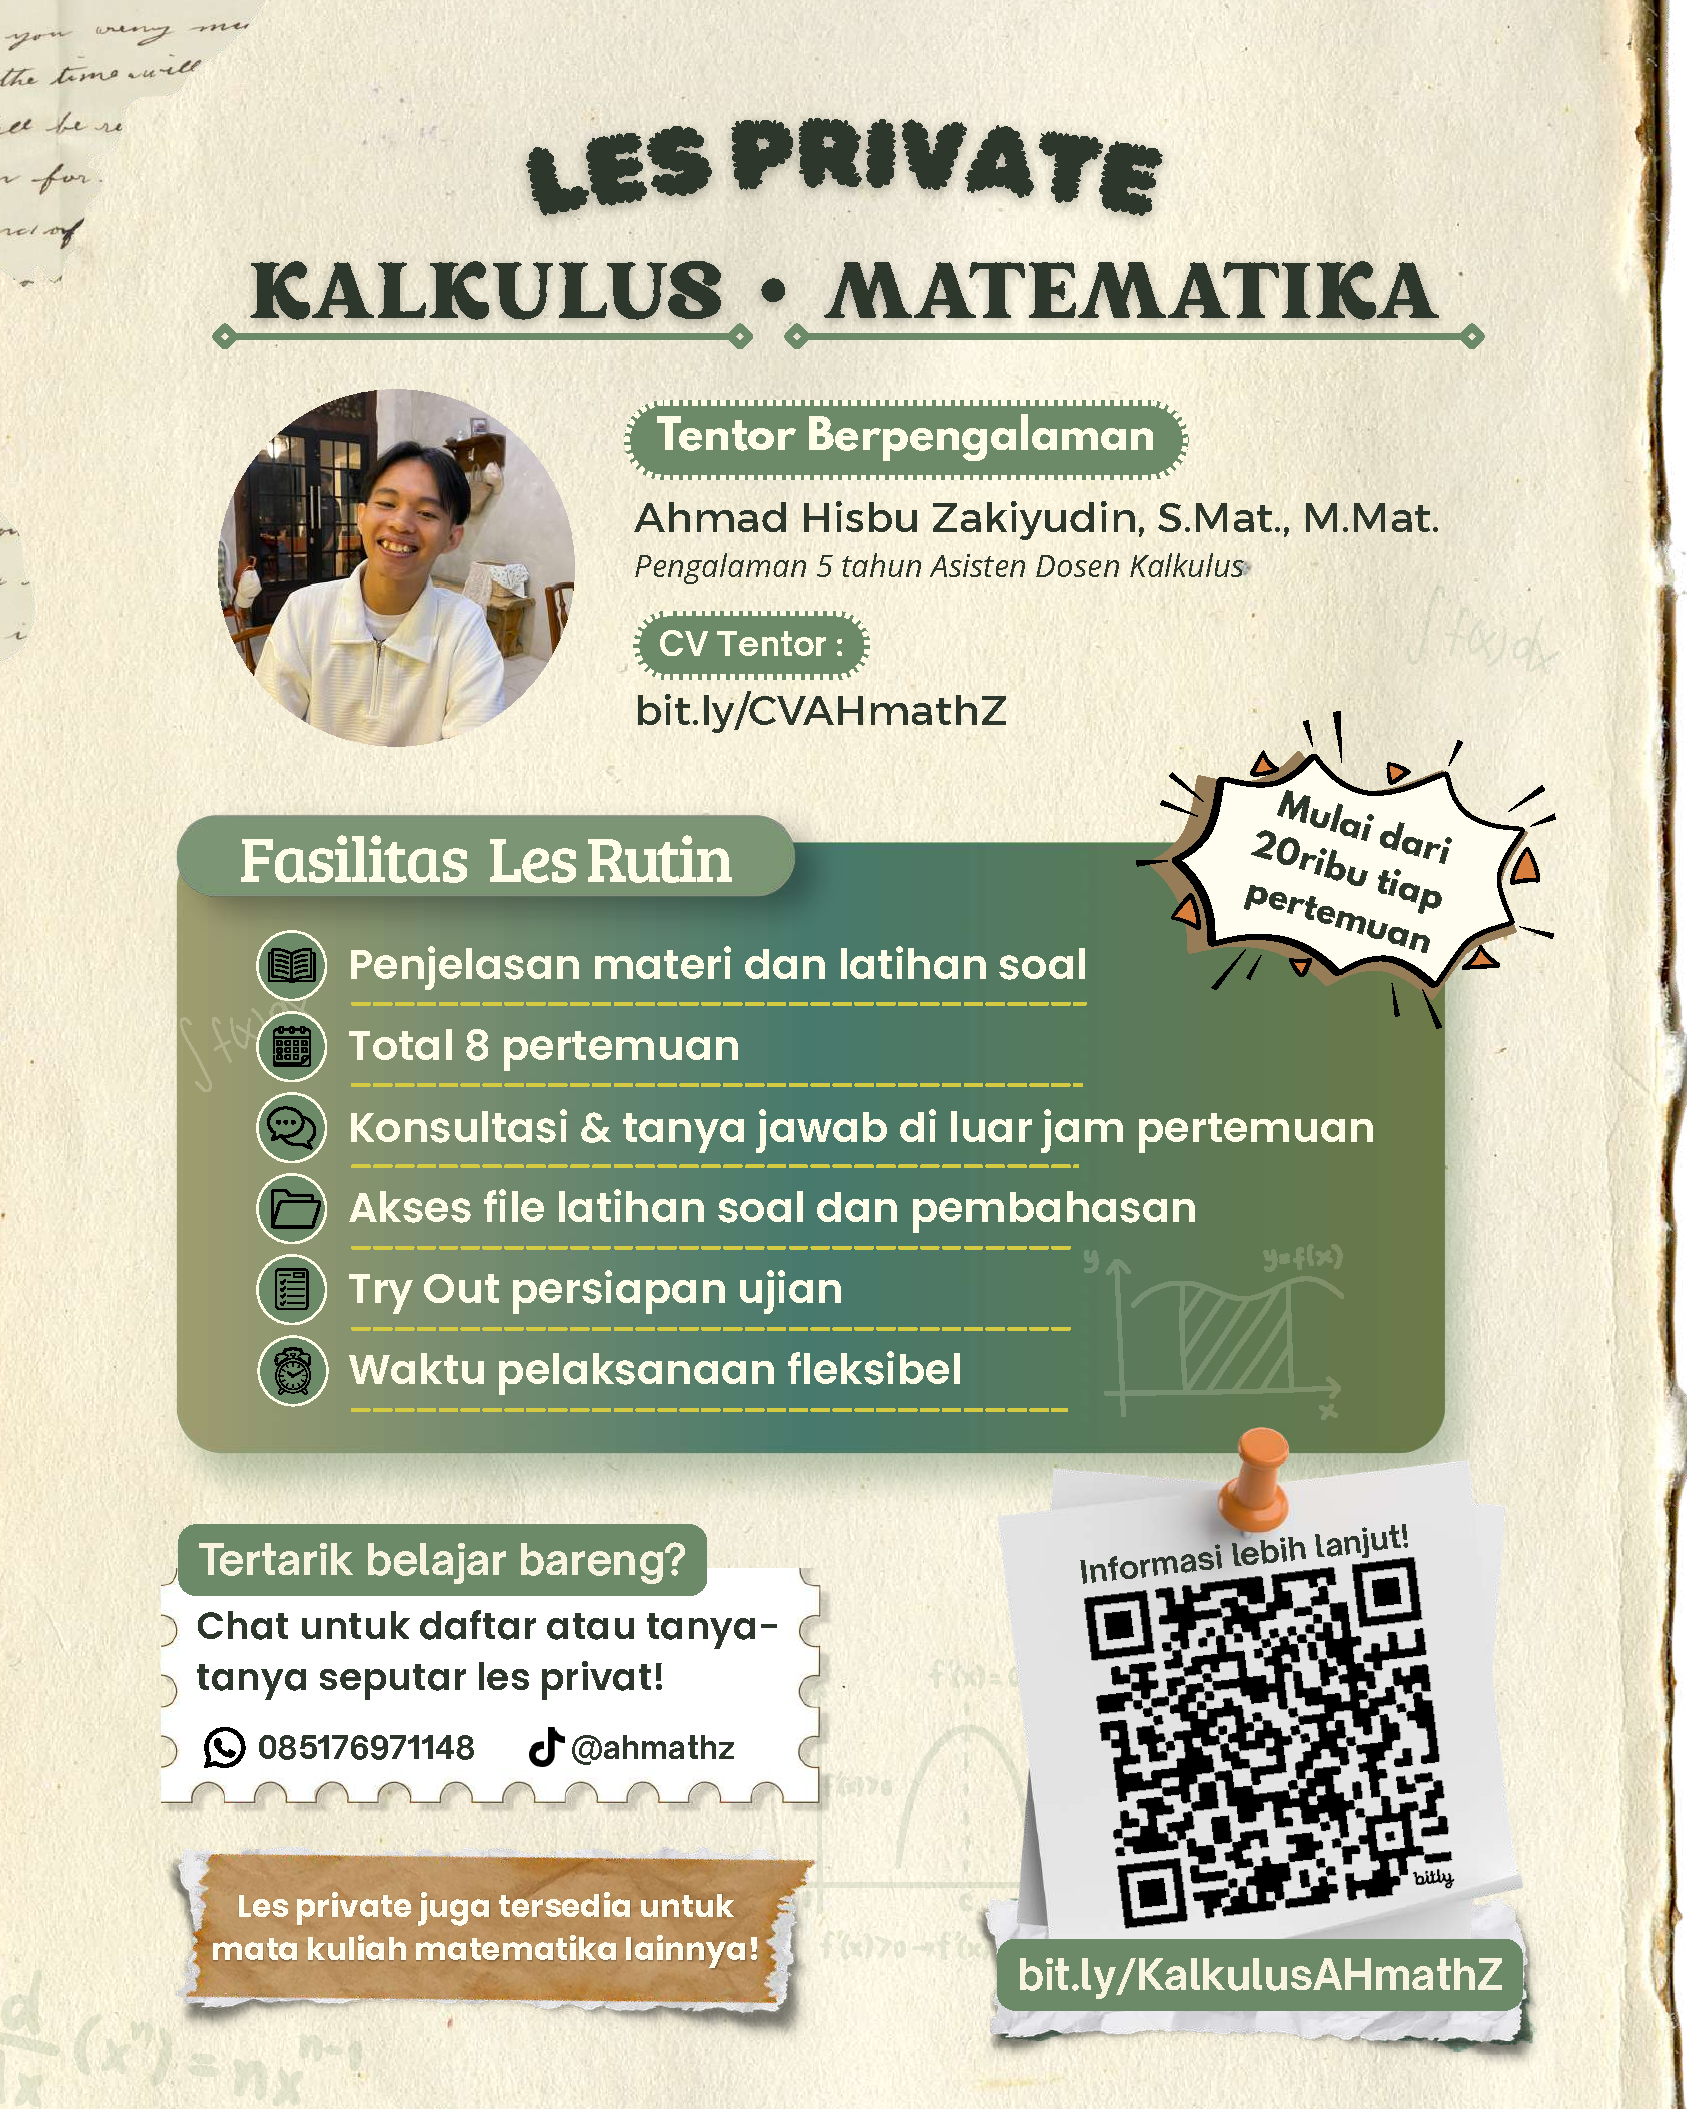
\includepdf[pages=-]{../ETS_Kalkulus_1_Th_2025-2026/les.pdf}

\end{document}
